\ifdefined\standalone 
\documentclass[12pt]{article}
\usepackage{graphicx}
\usepackage{float}
\usepackage[a4paper, margin=1in]{geometry}
\usepackage[utf8]{inputenc}
\usepackage{textcomp}
\usepackage{amsmath}
\usepackage{booktabs}
\usepackage{tikz}
\usepackage{enumitem}
\usetikzlibrary{decorations.pathmorphing,patterns}
\usepackage[hidelinks]{hyperref} % <- hypertext

\begin{document}
\fi

\section{Fixed heat flux boundary condition}
\label{case:rad_1d}


This verification case examines one-dimensional heat conduction in a slab subjected to a prescribed surface heat flux. A slab of thickness $4~\mathrm{cm}$ is initially at a uniform temperature of $T_{ini} = 27~^\circ\mathrm{C}$. The exposed surface is subjected to a constant incident heat flux of $q''_{\mathrm{ext}} = 2~\mathrm{kW\,m^{-2}}$. The material is assumed to be opaque, such that no in-depth radiation penetration occurs. The opposite surface is considered adiabatic, as illustrated in Figure~\ref{fig:rad1d_configuration}. The thermophysical properties of the material are summarized in Table~\ref{tab:phys_props_rad}.

The numerical results are validated against the analytical solution for transient heat conduction in a semi-infinite slab subjected to a constant surface heat flux, as presented by Incropera et al.~\cite{incropera_fundamentals_2007}. The analytical solution is given by:

\begin{equation}
T(z,t) - T_{ini} =
\frac{2 \varepsilon q''_{\mathrm{ext}}}{k}
\left( \frac{\alpha t}{\pi} \right)^{1/2}
\exp\left( -\frac{z^2}{4 \alpha t} \right)
-
\frac{\varepsilon q''_{\mathrm{ext}} z}{k}
\, \mathrm{erfc}\!\left( \frac{z}{2\sqrt{\alpha t}} \right)
\label{eq:T_xt}
\end{equation}
where $\alpha = k / (\rho c_p)$ is the thermal diffusivity, $\varepsilon$ is the surface emissivity, and $x$ denotes the distance from the exposed surface.


\begin{table}[H]
\centering
\caption{Thermophysical properties used in the simulation}
\label{tab:phys_props_rad}
\renewcommand{\arraystretch}{1.3}
\begin{tabular}{c c c c}
\hline
$k$ ($\mathrm{W\,m^{-1}\,K^{-1}}$) &
$c_p$ ($\mathrm{kJ\,kg^{-1}\,K^{-1}}$) &
$\rho$ ($\mathrm{kg\,m^{-3}}$) &
$\varepsilon$ ($-$) \\
\hline
0.186 & 1.764 & 380 & 1.0 \\
\hline
\end{tabular}
\end{table}

\begin{figure}[H]
\centering
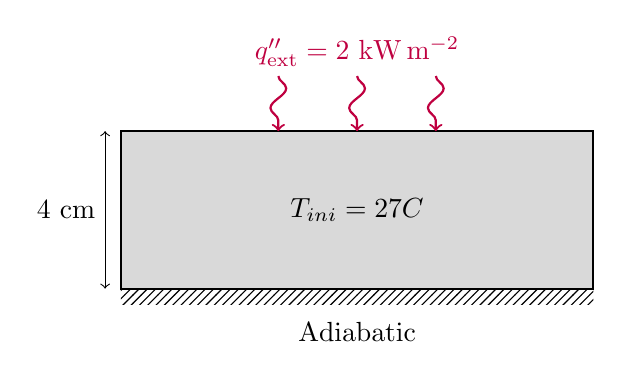
\begin{tikzpicture}[scale=1]
\draw[fill=gray!30,thick] (0,0) rectangle (6,2);
\node at (3,1) {$T_{ini}=27°C$};

\fill[pattern=north east lines] (0,-0.2) rectangle (6,0);
\node[below] at (3,-0.3) {Adiabatic};

\draw[<->] (-0.2,0) -- (-0.2,2);
\node[left] at (-0.2,1) {$4~\mathrm{cm}$};

\foreach \x in {1.8,2.8,3.8}
  \draw[purple,thick,->,decorate,decoration={snake,amplitude=1mm,segment length=5mm}]
  (\x+0.2,2.7) -- (\x+0.2,2);

\node[above,purple] at (3,2.7) { $q''_{\mathrm{ext}} = 2~\mathrm{kW\,m^{-2}}$};
\end{tikzpicture}
\caption{Schematic representation of the computational configuration.}
\label{fig:rad1d_configuration}
\end{figure}





\begin{figure}[H]
\centering
\includegraphics[width=0.6\textwidth]{radiation_1d.png}
\vspace{-0.4cm}
\caption{Temperature evolution at different depths inside the slab.}
\label{fig:rad_1d}
\end{figure}




\ifdefined\standalone
\bibliographystyle{unsrt}
\bibliography{radiation_1d}
\end{document}
\fi






